\documentclass[sigconf]{acmart}

% ---------- Required packages (ACM whitelist) ----------
\usepackage{graphicx}
\usepackage{subcaption}
\usepackage{amsmath}
\usepackage{booktabs}
\usepackage{multirow}
\usepackage{hyperref}

% ---------- Metadata ----------
\title{Enhancing [Task/Domain] via Novel Deep Autoencoder Architectures}

\author{Mluleki Wenkaba Mtande}
\affiliation{
  \institution{[Your Institution or Independent Researcher]}
  \city{}
  \country{}
}
\email{[mlumtande@gmail.com]}

\begin{abstract}
The RecSys Challenge 2025 promotes unified user modeling in e-commserce, asking participants to generate universal user representations from large-scale behavioral logs. These embeddings, built from millions of purchase, cart, and browsing events, are evaluated across multiple predictive tasks—both known and hidden—to assess their generalization ability. In this paper, we present our submission, which employs a novel autoencoder framework integrating residual connections, contrastive regularization, and curriculum noise. We highlight the practical and methodological challenges faced in developing universal representations, analyze performance across tasks, and reflect on how future RecSys challenges can further promote generalizable, robust, and application-agnostic user modeling.
\end{abstract}

\keywords{Deep Learning, Autoencoder, Representation Learning, [Domain], [Technique]}

\begin{document}

\maketitle

\section{Introduction}
Predictive analytics are fundamental to modern e-commerce, powering applications such as personalized recommendations, churn prediction, and propensity estimation. Traditionally, these tasks are approached independently, despite all relying on the same core resource: detailed logs of user behavior. This fragmentation can result in redundant modeling and limited generalizability.

The RecSys Challenge 2025 \cite{recsys2025} directly addresses this issue by promoting a unified approach to behavior modeling. Organized by Synerise and an international team of academic collaborators, the challenge introduces the concept of \emph{Universal Behavioral Profiles}: compact user representations meant to capture essential patterns across diverse interactions—purchases, cart actions, page views, and search queries. The central objective is to produce embeddings that perform robustly across multiple downstream tasks, both disclosed and undisclosed, reflecting their generalization power.

Participants are provided with a massive, real-world dataset containing millions of multi-type user events. Rather than optimizing for a single target, submitted embeddings are evaluated in several predictive tasks—including churn and product propensity prediction—using a composite score that aggregates performance across all tasks. This setup not only emphasizes robust, transferable representation learning, but also mirrors real-world business requirements, where unified user profiles support a range of analytics and decision-making systems.

In this paper, we present our approach to the challenge, based on an advanced autoencoder architecture combining residual connections, contrastive learning, and curriculum noise. We discuss the practical challenges of universal representation learning, analyze empirical results across tasks, and reflect on the implications for future research in recommender systems and behavior modeling.

\subsection{Problem Statement}
The core problem addressed in the RecSys Challenge 2025 is the development of \emph{Universal Behavioral Profiles}: user representations that effectively encode past interactions—such as purchases, cart modifications, searches, and page visits—for large-scale e-commerce platforms. Unlike traditional approaches that train distinct models for each predictive task, the challenge requires participants to learn a single, compact embedding per user that generalizes across a range of downstream applications.

Given a dataset comprising millions of multi-type user events, the objective is to construct user embeddings that maximize predictive performance not only on known tasks, such as churn and product propensity prediction, but also on undisclosed, hidden tasks provided by the organizers. The quality of these universal embeddings is measured by aggregating their performance across all evaluation tasks using a composite score.

The key technical challenge lies in learning representations that are robust, transferable, and capable of capturing both broad behavioral patterns and fine-grained individual preferences. Participants must address issues of scalability, data heterogeneity, and the need for embeddings that retain generalizable information relevant to diverse business objectives.
\subsection{Dataset}
The dataset provided in the RecSys Challenge 2025 comprises over 168 million events generated by approximately 19 million users in a real-world e-commerce platform. Each event is timestamped and belongs to one of several categories: product purchase, add-to-cart, remove-from-cart, page visit, or search query. The data presents unique challenges, including high user and item cardinality, varying interaction frequencies, and temporal sparsity, making effective representation learning both essential and nontrivial.

\label{sec:related}
\section{Related Work}

Autoencoders have become a foundational approach for unsupervised representation learning in domains such as recommender systems, user modeling, and behavioral analytics~\cite{Hinton2006, Vincent2008, Kingma2014, Sedhain2015}. By compressing high-dimensional input data into lower-dimensional latent representations, autoencoders can uncover underlying structure and facilitate a wide range of downstream predictive tasks. Numerous architectural enhancements have been proposed, including denoising objectives~\cite{Vincent2008}, variational formulations~\cite{Kingma2014}, and residual connections~\cite{He2016ResNet, Mao2016}. These innovations address issues such as information loss, vanishing gradients, and improved robustness to noise.

Beyond autoencoders, the field of representation learning has been shaped by contrastive learning~\cite{Oord2018, Chen2020SimCLR}, self-supervised objectives, and metric learning, all of which aim to produce embeddings that capture meaningful similarities and differences in the data. In recent recommender systems research, combining autoencoder architectures with contrastive or self-supervised regularization has shown improved generalization and task transfer~\cite{Zhou2020S3Rec, Zhan2022CLAES}. However, learning representations that remain robust across heterogeneous event types and diverse predictive tasks, as required in the RecSys Challenge 2025, remains an open research problem.

\section{Proposed Method}
\label{sec:method}
\subsection{Feature Engineering Pipeline}
Our feature engineering pipeline is designed to transform raw, heterogeneous event logs into a rich set of user-level features that capture temporal dynamics, behavioral diversity, conversion tendencies, and nuanced patterns of online shopping. The main components are:

\begin{itemize}
  \item \textbf{Temporal Features:} 
  To capture daily and weekly periodicities, we apply sine and cosine transformations to the hour-of-day and day-of-week variables, enabling the model to recognize cyclical user habits (e.g., weekend vs. weekday shopping). We extract each user’s peak activity hours and compute their activity momentum, reflecting trends in engagement over time (e.g., increasing or declining activity).

  \item \textbf{Session Features:} 
  Sessions are segmented using a 30-minute inactivity window. For each user, we calculate statistics on session duration (mean, variance), inter-session intervals, and the distribution of activity across parts of the day (morning, afternoon, evening, night). The session burst ratio quantifies how often users exhibit dense bursts of activity versus more sporadic engagement.

  \item \textbf{Behavioral Features:}
  We measure the diversity of browsing and purchasing by computing entropy and Gini coefficients over interacted categories. SKU exploration rates capture the ratio of unique items viewed to total actions, indicating novelty-seeking tendencies. Novelty-seeking itself is also directly quantified, reflecting users’ inclination to explore new content or products.

  \item \textbf{Conversion Features:}
  Conversion efficiency is evaluated through cart abandonment rates, the proportion of search queries leading to purchases, and immediate (same-session) conversion rates. Price sensitivity is measured by observing changes in purchase likelihood across price ranges.

  \item \textbf{Advanced Behavioral Metrics:}
  Beyond standard features, we introduce several novel, high-level metrics:
    \begin{itemize}
      \item \textit{Price Sensitivity Curve:} Models how purchase probability varies with price, using binned regression and elasticity calculations to profile value-driven behavior.
      \item \textit{Exploration-Exploitation Balance:} Quantifies the user's balance between discovering new SKUs and revisiting familiar ones, using cumulative curves of unique SKUs explored over time.
      \item \textit{Purchase Journey Analysis:} Analyzes the efficiency of a user’s progression from search to visit, cart, and purchase, constructing compound metrics that summarize funnel conversion effectiveness.
      \item \textit{Session Progression Patterns:} Compares the types and frequencies of events at different phases of sessions, identifying shifts in behavior from session start to end.
      \item \textit{Temporal Shopping Patterns:} Detects periodic shopping intervals and category-specific cycles, capturing both regular and sporadic purchasing habits.
      \item \textit{Behavioral Segmentation:} Employs binary indicator features to identify archetypal behavioral segments (such as researchers, browsers, decisive buyers, or loyal customers), supporting downstream personalization and analysis.
    \end{itemize}
\end{itemize}\vspace{-1em}
This comprehensive feature engineering pipeline ensures that the resulting user representations incorporate both granular and high-level behavioral signals, facilitating robust generalization across a diverse set of predictive tasks as required by the RecSys Challenge 2025. The inclusion of advanced metrics and segmentation enables deeper modeling of intent, preferences, and evolving user journeys in large-scale e-commerce contexts.
\subsection{Model Architecture Overview}

\begin{figure}[t]
  \centering
  % Replace with actual diagram or export from Figma/draw.io as PDF/PNG for submission
  \includegraphics[width=0.9\linewidth]{autoencoder_pipeline_diagram.png}
  \caption{Overview of the universal user profile generation pipeline. Engineered user features are transformed via a deep residual autoencoder with contrastive and noise-based regularization to yield universal embeddings.}
  \label{fig:architecture}
\end{figure}

As shown in Figure~\ref{fig:architecture}, our pipeline begins by processing raw behavioral logs into a comprehensive set of engineered features (see Section~X.X). These features—encompassing temporal cycles, session statistics, conversion rates, and advanced behavioral metrics—form a high-dimensional input vector for each user.

\textbf{Encoder:}  
The encoder comprises a stack of four fully connected layers with dimensions [512, 256, 128, 64], each followed by batch normalization and GELU activation. Residual skip connections are added after each layer to facilitate gradient flow and retain both high-level and fine-grained information from the input features.

\textbf{Latent Layer:}  
The bottleneck layer (dimension 32 or 64, depending on hyperparameter sweep) serves as the compact universal behavioral profile for each user. This latent representation is optimized not only for input reconstruction but also for generalization across downstream tasks.

\textbf{Decoder:}  
The decoder mirrors the encoder structure, expanding the latent vector back to the original feature dimension. This reconstruction objective ensures the embedding retains as much salient information from the original behavioral data as possible.

\textbf{Loss Functions:}  
Our training objective combines three terms: (1) mean squared error (MSE) for feature reconstruction, (2) a lightweight InfoNCE contrastive loss computed between latent vectors of augmented (noisy) user feature pairs, and (3) L2 regularization on the latent embeddings. The total loss is  
\[
\mathcal{L}_{total} = \mathcal{L}_{rec} + \lambda_{con}\mathcal{L}_{con} + \lambda_{L2}\|\mathbf{z}\|_2^2
\]  
where $\lambda_{con}$ and $\lambda_{L2}$ are weighting coefficients determined via grid search.

\textbf{Curriculum Noise:}  
To improve robustness, Gaussian noise is added to the input features during training, with the noise variance annealed linearly from $\sigma=0.10$ to $\sigma=0.02$ over epochs. This encourages the autoencoder to learn stable, generalizable patterns before focusing on subtle, task-specific details.

\textbf{Integration with Feature Engineering:}  
The success of the model is closely linked to the expressiveness of the engineered features. High-level constructs—such as session progression, price sensitivity, and behavioral segmentation—not only expand the representational capacity of the latent embeddings but also promote transferability across varied prediction targets (e.g., churn, propensity, category preference). The autoencoder thus serves as a powerful information compressor, distilling hundreds of heterogeneous signals into a unified, compact profile for each user.

By combining advanced feature engineering with a robust, regularized autoencoder architecture, our system produces user embeddings that meet the RecSys Challenge 2025’s goals of universal, high-utility representation.

\subsection{Model Architecture Overview}

\begin{figure}[t]
  \centering
  % Replace with actual diagram or export from Figma/draw.io as PDF/PNG for submission
  \includegraphics[width=0.9\linewidth]{images/autoencoder_pipeline_diagram.png}
  \caption{Overview of the universal user profile generation pipeline. Engineered user features are transformed via a deep residual autoencoder with contrastive and noise-based regularization to yield universal embeddings.}
  \label{fig:architecture}
\end{figure}

As shown in Figure~\ref{fig:architecture}, our pipeline begins by processing raw behavioral logs into a comprehensive set of engineered features (see Section~X.X). These features—encompassing temporal cycles, session statistics, conversion rates, and advanced behavioral metrics—form a high-dimensional input vector for each user.

\textbf{Encoder:}  
The encoder comprises a stack of four fully connected layers with dimensions [512, 256, 128, 64], each followed by batch normalization and GELU activation. Residual skip connections are added after each layer to facilitate gradient flow and retain both high-level and fine-grained information from the input features.

\textbf{Latent Layer:}  
The bottleneck layer (dimension 32 or 64, depending on hyperparameter sweep) serves as the compact universal behavioral profile for each user. This latent representation is optimized not only for input reconstruction but also for generalization across downstream tasks.

\textbf{Decoder:}  
The decoder mirrors the encoder structure, expanding the latent vector back to the original feature dimension. This reconstruction objective ensures the embedding retains as much salient information from the original behavioral data as possible.

\textbf{Loss Functions:}  
Our training objective combines three terms: (1) mean squared error (MSE) for feature reconstruction, (2) a lightweight InfoNCE contrastive loss computed between latent vectors of augmented (noisy) user feature pairs, and (3) L2 regularization on the latent embeddings. The total loss is  
\[
\mathcal{L}_{total} = \mathcal{L}_{rec} + \lambda_{con}\mathcal{L}_{con} + \lambda_{L2}\|\mathbf{z}\|_2^2
\]  
where $\lambda_{con}$ and $\lambda_{L2}$ are weighting coefficients determined via grid search.

\textbf{Curriculum Noise:}  
To improve robustness, Gaussian noise is added to the input features during training, with the noise variance annealed linearly from $\sigma=0.10$ to $\sigma=0.02$ over epochs. This encourages the autoencoder to learn stable, generalizable patterns before focusing on subtle, task-specific details.

\textbf{Integration with Feature Engineering:}  
The success of the model is closely linked to the expressiveness of the engineered features. High-level constructs—such as session progression, price sensitivity, and behavioral segmentation—not only expand the representational capacity of the latent embeddings but also promote transferability across varied prediction targets (e.g., churn, propensity, category preference). The autoencoder thus serves as a powerful information compressor, distilling hundreds of heterogeneous signals into a unified, compact profile for each user.

By combining advanced feature engineering with a robust, regularized autoencoder architecture, our system produces user embeddings that meet the RecSys Challenge 2025’s goals of universal, high-utility representation.



\subsection{Training Strategy}

\section{Experimental Setup}
\label{sec:experiments}
\subsection{Datasets and Preprocessing}
\subsection{Baselines}
\subsection{Evaluation Metrics}

\section{Results and Discussion}
\subsection{Quantitative Results}
\subsection{Ablation Study}
\subsection{Qualitative Analysis}
\subsection{Discussion}

\section{Conclusion and Future Work}
\label{sec:conclusion}
\subsection{Summary of Findings}
\subsection{Limitations}
\subsection{Future Directions}

\begin{acks}
[Optional: Funding, collaborators, etc.]
\end{acks}

\bibliographystyle{ACM-Reference-Format}
\bibliography{references}

\end{document}
